\section{Dimensionality Reduction \& Noise Filtering}
\label{sec:dim_reduction}

The HICO image cube is converted to a matrix on the form L x N, 
with $L$ spectral bands rows, and $N = WH$ columns. 

\subsection{What is dimensionality reduction?}

Dimensionality reduction is the act of reducing the amount of random variables 
to consider in for instance machine learning and statistics, involving feature 
selection and feature extraction. Thus making the data smaller and making 
analyzing it faster and easier. 

Considering \cref{fig:point_spectra}, we see that there are quite a few similarities 
in the spectra of the various points. Looking at the two points in the water (shallow 
and deep), we see that the spectra are almost identical to each other for wavelengths 
between around 400 - 470nm, except for the clear difference in the amplitude. Even the 
spectra for the vegetation seem to share this characteristic. For wavelengths between 
470 - 800nm all spectra seem to have unique signatures, until the two points in the 
water again seem to share quite similar spectra for wavelengths over 800nm, with only 
small variations between the two. An other thing to consider is the fact that the 
atmospheric correction algorithm used in \cref{sec:atmoshperic_cor} is invalid for 
wavelengths outside the range 438 - 730nm, so these invalid bands can be dropped. 
Thus there seems to be some opportunities to reduce the dimensionality in the 
spectral dimensions for the aforementioned wavelengths.

In the spatial direction, we could for instance ignore all of the landmass, as we 
are only interested in looking at the water. This can be done as described in 
\cref{sec:landmask}, where all points on land are simply set to 0, thus reducing the 
spatial dimension significantly by removing a big chunk of the image. The spatial 
dimension can be reduced further by doing a nearest neighbor approach to cluster data 
together, for instance in the deep water in the upper left part of the image, \cref{fig:pseudo_rgb}, 
where a portion of the ocean seem to be very similar in appearance. This can be done 
using for example k-means clustering, as described previously in \cref{sec:classify}. 

\subsection{Principal Component Analysis (PCA)}

PCA is a dimensionality reduction technique that transforms the columns of a dataset 
into a new set features, by finding a new set of directions that explain the maximum 
variability in the data \cite{prabhakaran2019}. These new coordinate axes/directions 
are known as the Principal Components (PCs). The dataset columns contains the amount 
of variance of the data, computing the PCs will help explain the vast information in 
the original data in a fewer amount of columns. 

If we do PCA on a matrix $X$ with 100 rows and 1000 columns, using 10 basis vectors 
the PCA components will have the following shapes:

\begin{itemize}
    \item Original data shape:  (100, 1000)
    \item PCA dataframe shape:  (10, 1000)
    \item PCA weights shape:  (100, 10)
\end{itemize}

Meaning we have 10 weights per column, $10 \times 1000 = 10000$ weights in total. 

The weights in the PCA is the eigenvectors of X. Each principal component is the dot 
product of its weights and the mean-centered data (each column of X is subtracted from 
its own mean, so the mean of each column is zero). 

\begin{equation}
    PC_i = weights \cdot X_{meancentered}
\end{equation}


\subsection{How does dimensionality reduction via PCA afect classification?}

PCA was implemented using the existing PCA algorithm from \textit{sklearn.decomposition}. 
First we convert the HICO image cube into matrix form, as described in \cref{sec:dim_reduction}, 
We then run the PCA with $P = 10$ principal components on this data matrix, returning 
an $P \times N$ size matrix representing the compressed data. That is $10 \times 250000$ in size, 
down from $100 \times 250000$, a ten times reduction in size. Looking at the variance 
of the 10 principle components, shown in \cref{eq:pca_var} and plotted in \cref{fig:pca_var}, we 
clearly see that all the variance in the dataset is contained in the first 3 principle components, 
with a total of 91\% being in the first component alone. 
Thus we could potentially reduced the dataset even further, down to only 3 components, without 
losing any significant data. 

\begin{equation}
    \label{eq:pca_var}
    [0.91, 0.08, 0.01, 0,   0,   0,   0,   0,   0,   0,  ]
\end{equation}

Running K-means clustering on the PCA compressed data we notice a great increase in performance. 
Clustering the compressed data, running kmeans for 1-10 classes and max 50 iterations, 
now only takes about 53 seconds, compared to the 128 seconds 
it takes to classify the uncompressed data. The resulting clustering can be seen in 
\cref{fig:pca_kmean}, which looks more or less identical to the clustering from the 
original data in \cref{fig:kmean}. From the cluster means plot (right on \cref{fig:pca_kmean}) 
we see that there is almost no variation for $PC > 2$, except for the one outlier.

Reducing the number of PCs to $P = 3$ we get even faster performance, using only 
22 seconds to do the classification. The resulting image is identical to \cref{fig:pca_kmean}, 
as all the principal component containing all the variance/information in the dataset is still kept, 
even though the data is significantly more compressed. 

If the PCA is done using 100 principle components instead, we get a negative impact on the 
performance. Now the same kmeans clustering spends 145 seconds, while giving the same 
results as with 10 or even 3 components.

Turning P even lower, to $P = 1$, the kmeans finishes after only 15 seconds. However, we 
have lost some information. It is no longer possible to classify the data correctly as we 
have removed too much information. Some noticeable differences here is the inability to 
separate the different classes of the ocean, as there is no longer individual classes for 
shallow and deep water, but just one class in total for the ocean. Thus, this data is now 
useless for our purposes. 

\begin{figure}
    \centering
    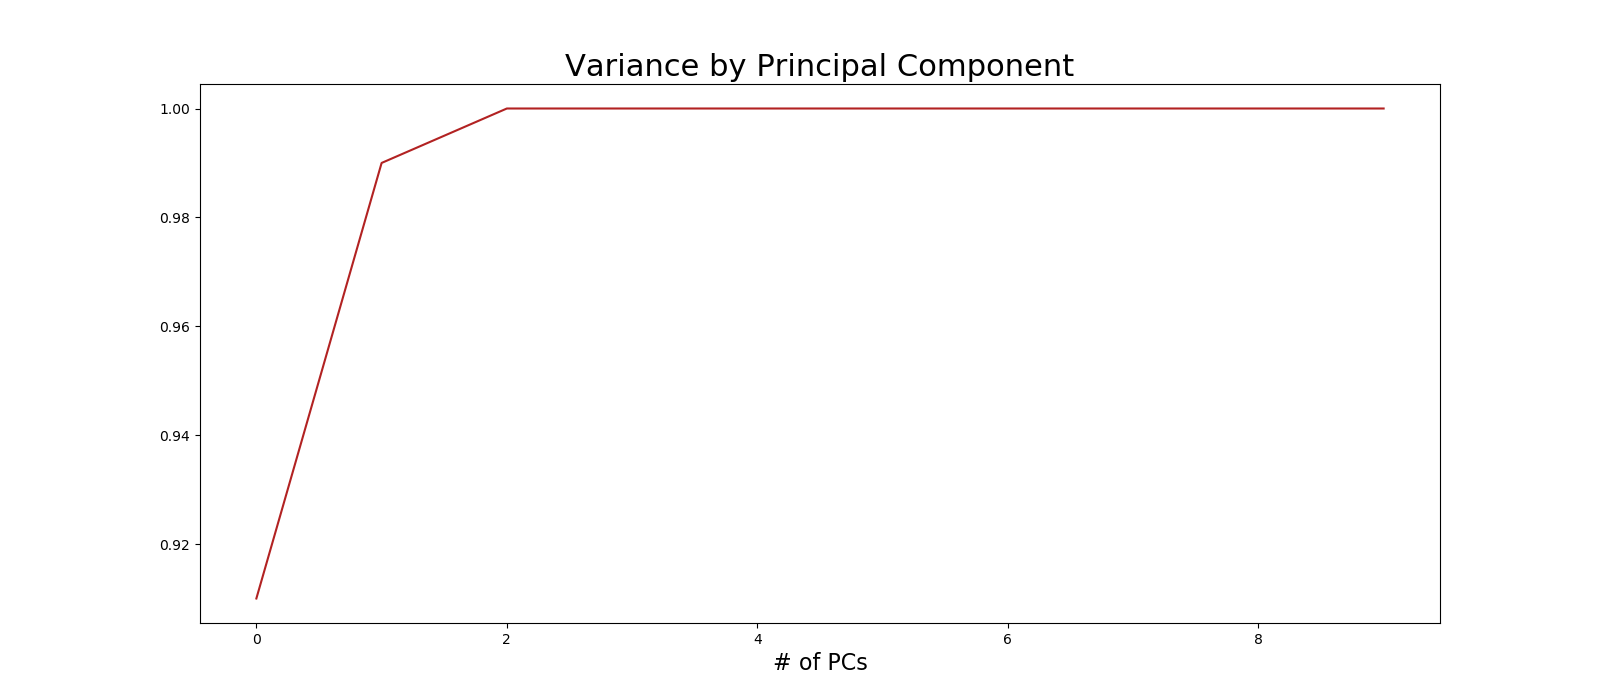
\includegraphics[width=\textwidth]{../fig/pca/variance_cumsum.png}
    \caption{Plotting the cumulative variance of the principal components}
    \label{fig:pca_var}
\end{figure}

\begin{figure}
    \centering
    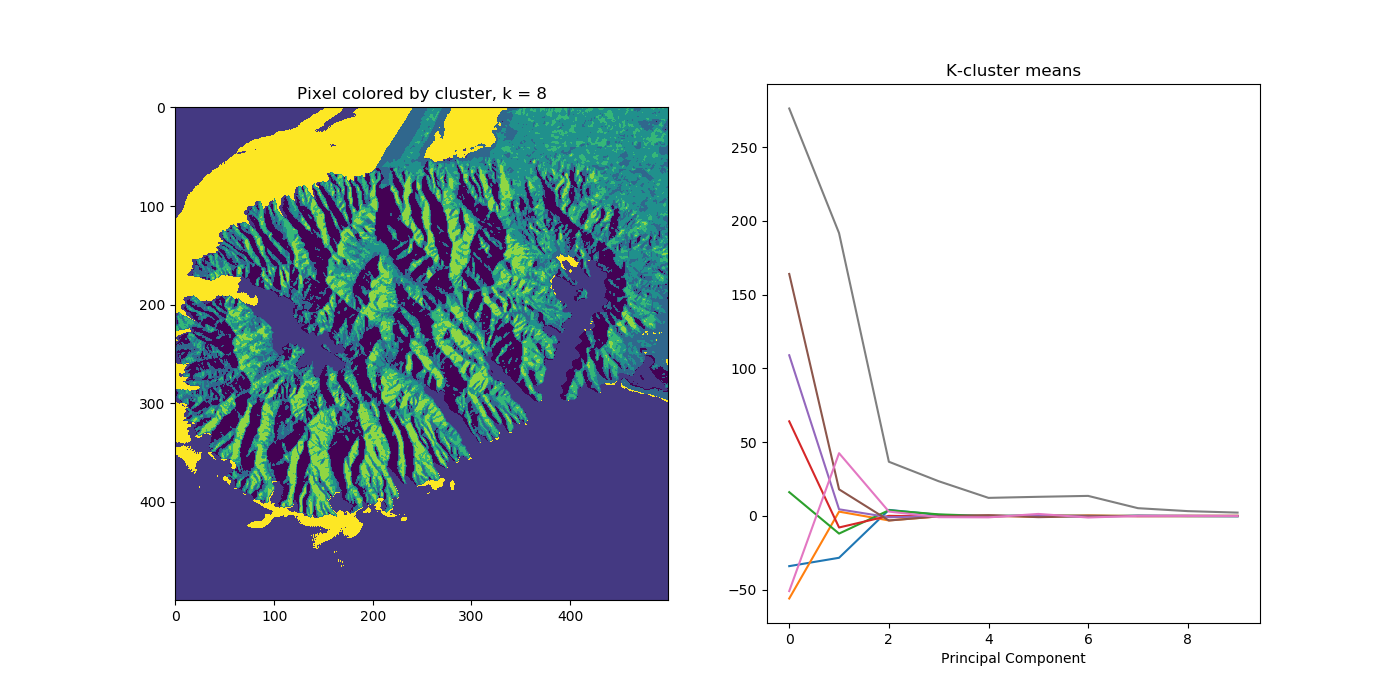
\includegraphics[width=\textwidth]{../fig/kmean/PCA_8}
    \caption{K-means classification performed on the PCA compressed data, using 10 Principal Components.}
    \label{fig:pca_kmean}
\end{figure}


\subsection{Maximum Noise Fraction}

\subsection{Maximum Noise Fraction on HICO noisy}

\subsection{Discuss your results}

\subsection{How can we best use the subspace?}
